% !TEX program = pdflatex
%Numerical Experiment_3
\documentclass[10pt,a4paper]{article}
\usepackage[UTF8]{ctex}
\usepackage{bm}
\usepackage{amsmath}
\usepackage{amssymb}
\usepackage{graphicx}
\usepackage{subfigure}
%\usepackage{geometry}
%\geometry{a4paper,left=.3cm,right=.3cm,top=1cm,bottom=1.5cm}
\usepackage{float}
\usepackage{multirow}
\usepackage{listings}
\usepackage[framed,numbered,autolinebreaks,useliterate]{mcode}
\usepackage{textcomp}
\title{数值试验三报告}
\author{陈稼霖 \and 45875852}
\date{2019.5.23}
\begin{document}
\maketitle
\section*{一、体会数值方法的不稳定性对数值结果的影响}
分别用显式和隐式欧拉法求解$y'=-50y,y(0)=100$.\\
1. 取$h=0.05,0.04,0.03,\cdots$ 用显式欧拉法求解,当步长$h$取到多少时,数值解开始出现不稳定?\\
解:此问题的解析解为
\[
y=100e^{-50x}
\]
对于模型问题应用显式欧拉公式有
\[
y_{n+1}=y_n+hy'_k=(1-50h)y_n
\]
设在$x_n$处误差为$\varepsilon_n$,则有
\begin{gather*}
y_{n+1}+\varepsilon_{n+1}=(1+h\lambda)(y_n+\varepsilon_n)\\
\Longrightarrow\varepsilon_{n+1}=(1-50h)\varepsilon_n
\end{gather*}
要保证稳定性,则需
\begin{gather*}
|\frac{\varepsilon_{n+1}}{\varepsilon_n}|=|1-50h|\leq1\\
\Longrightarrow0\leq h\leq\frac{1}{25}=0.04
\end{gather*}
故通过理论预测,当步长$h>0.04$时,数值解开始出现不稳定。\\
下通过数值实验验证:

取$h=0.05$,得数值解及其误差如图\ref{1_1_1},发现数值解不稳定。
\begin{figure}[ht]
\centering
\subfigure[数值解与解析解]{
\begin{minipage}{0.48\textwidth}
\centering
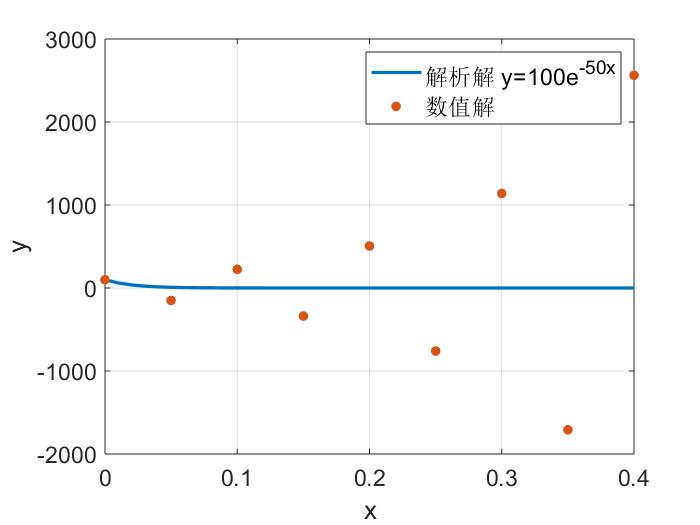
\includegraphics[width=6cm]{ExplEular_1_1_1.jpg}
\end{minipage}}
\subfigure[误差绝对值$\varepsilon_n$随迭代次数$n$变化的关系]{
\begin{minipage}{0.48\textwidth}\centering
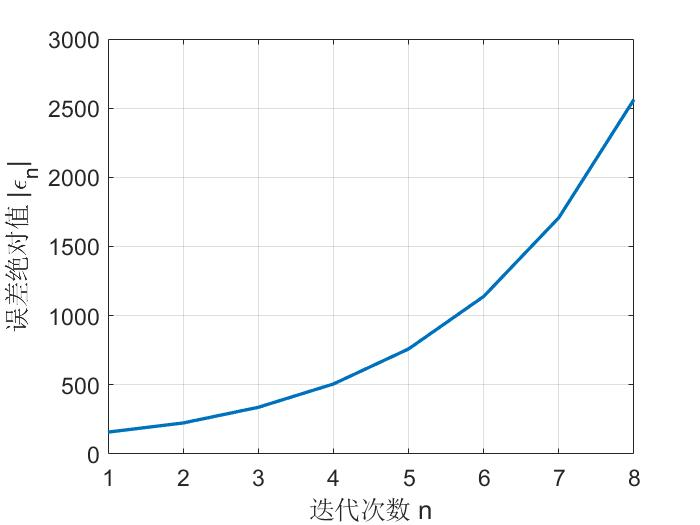
\includegraphics[width=6cm]{Error_1_1_1.jpg}
\end{minipage}}
\caption{$h=0.05$时的数值解及其误差}\label{1_1_1}
\end{figure}
\newpage

取$h=0.04$,得数值解及其误差如图\ref{1_1_2},发现数值解稳定。
\begin{figure}[ht]
\centering
\subfigure[数值解与解析解]{
\begin{minipage}{0.48\textwidth}
\centering
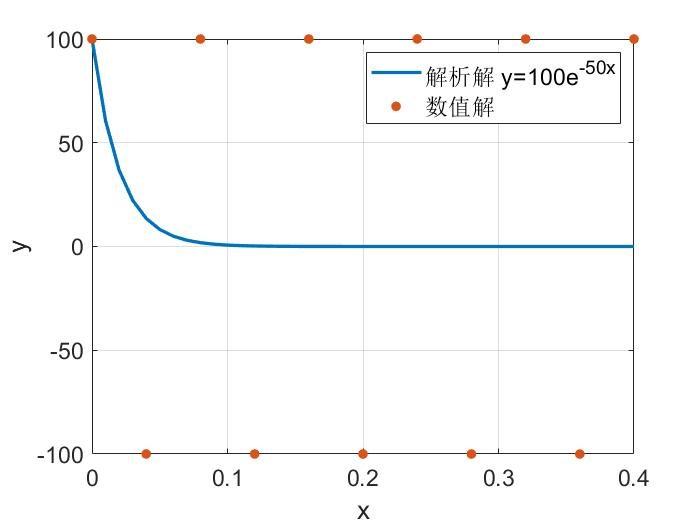
\includegraphics[width=6cm]{ExplEular_1_1_2.jpg}
\end{minipage}}
\subfigure[误差绝对值$\varepsilon_n$随迭代次数$n$变化的关系]{
\begin{minipage}{0.48\textwidth}\centering
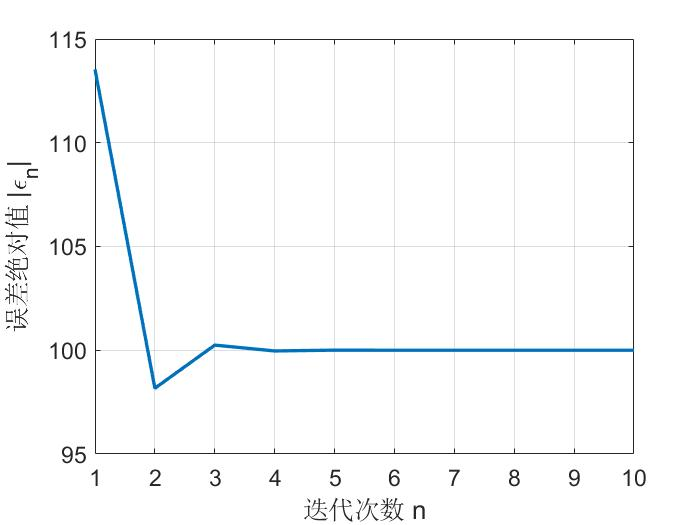
\includegraphics[width=6cm]{Error_1_1_2.jpg}
\end{minipage}}
\caption{$h=0.04$时的数值解及其误差}\label{1_1_2}
\end{figure}
\newpage

取$h=0.03$,得数值解及其误差如图\ref{1_1_3},发现数值解稳定。
\begin{figure}[ht]
\centering
\subfigure[数值解与解析解]{
\begin{minipage}{0.48\textwidth}
\centering
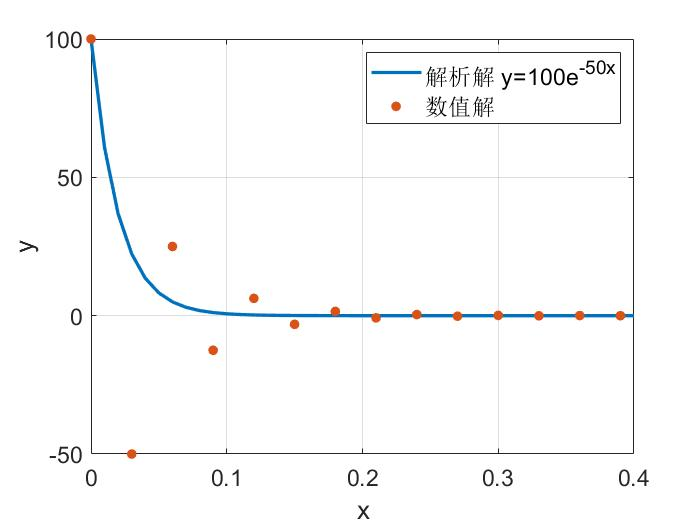
\includegraphics[width=6cm]{ExplEular_1_1_3.jpg}
\end{minipage}}
\subfigure[误差绝对值$\varepsilon_n$随迭代次数$n$变化的关系]{
\begin{minipage}{0.48\textwidth}\centering
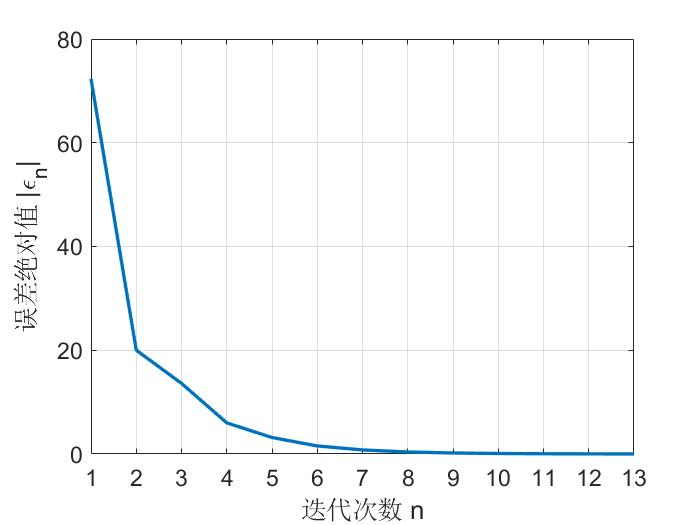
\includegraphics[width=6cm]{Error_1_1_3.jpg}
\end{minipage}}
\caption{$h=0.03$时的数值解及其误差}\label{1_1_3}
\end{figure}

取$h=0.01$,得数值解及其误差如图\ref{1_1_4},发现数值解稳定。
\begin{figure}[ht]
\centering
\subfigure[数值解与解析解]{
\begin{minipage}{0.48\textwidth}
\centering
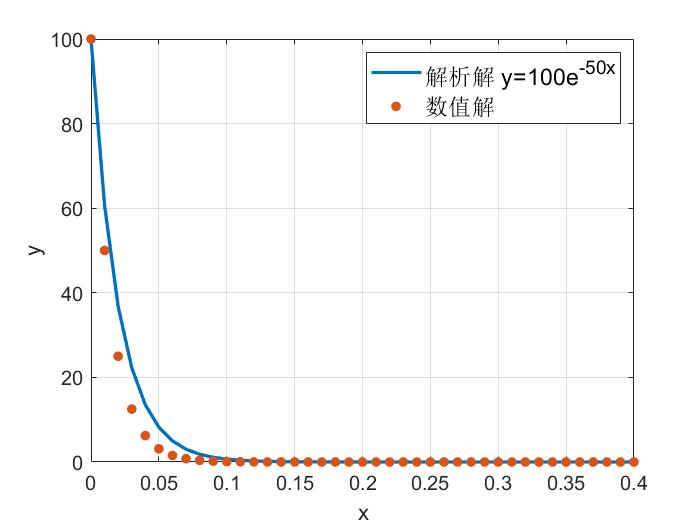
\includegraphics[width=6cm]{ExplEular_1_1_4.jpg}
\end{minipage}}
\subfigure[误差绝对值$\varepsilon_n$随迭代次数$n$变化的关系]{
\begin{minipage}{0.48\textwidth}\centering
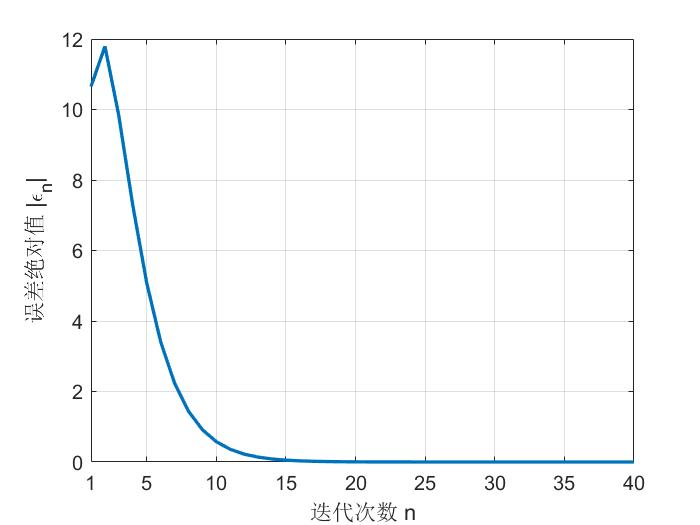
\includegraphics[width=6cm]{Error_1_1_4.jpg}
\end{minipage}}
\caption{$h=0.01$时的数值解及其误差}\label{1_1_4}
\end{figure}

综上,当取到步长$h>0.04$时,数值解开始出现不稳定,理论预测与数值实验相符。\\

2. 用隐式欧拉法求解上述问题,数值解会出现不稳定吗?\\
解:不会。\\
对于上述模型问题应用隐式欧拉公式有
\begin{gather*}
y_{n+1}=y_n+hy'_{n+1}=y_n-50hy_{n+1}\\
\Longrightarrow y_{n+1}=\frac{1}{1+50h}y_n
\end{gather*}
设在$x_n$处误差为$\varepsilon_n$,则有
\begin{gather*}
y_{n+1}+\varepsilon_{n+1}=\frac{1}{1+50h}(y_n+\varepsilon_n)\\
\Longrightarrow\varepsilon_{n+1}=\frac{1}{1+50h}\varepsilon_n
\end{gather*}
对于$\forall h>0$,都有
\[
|\frac{\varepsilon_{n+1}}{\varepsilon_n}|=|\frac{1}{1+50h}|<1
\]
故用隐式欧拉法求解上述问题,数值解不会出现不稳定。\\

\section*{二、体会算法的保结构性}
对一阶常微分方程组
\[
\left\{\begin{array}{ll}
y'(t)=-2x(t)\\
x'(t)=\frac{9}{2}y(t)\\
x(0)=3,&y(0)=2
\end{array}\right.
\]
分别用梯形法、Eular法,四阶Runge--Kutta法求解其数值解,并观察相平面中的轨迹。哪些方法求得的结果能保持相平面中轨迹不变。\\
解:用梯形法求解其数值解,相平面中的轨迹如图\ref{2_1},发现相平面中轨迹不变。
\begin{figure}[h]
\centering
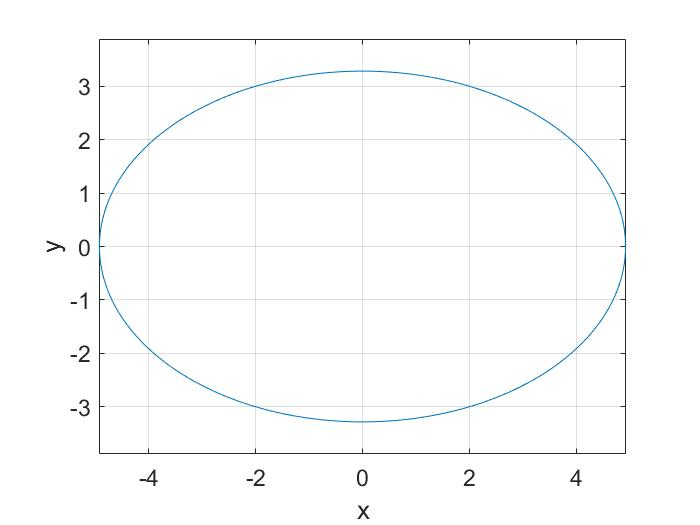
\includegraphics[width=8cm]{Trapezoid_2.jpg}
\caption{梯形法求得的相平面中的轨迹}\label{2_1}
\end{figure}

用显式Eular法求解其数值解,相平面中的轨迹如图\ref{2_2},发现相平面中轨迹偏离。
\begin{figure}[h]
\centering
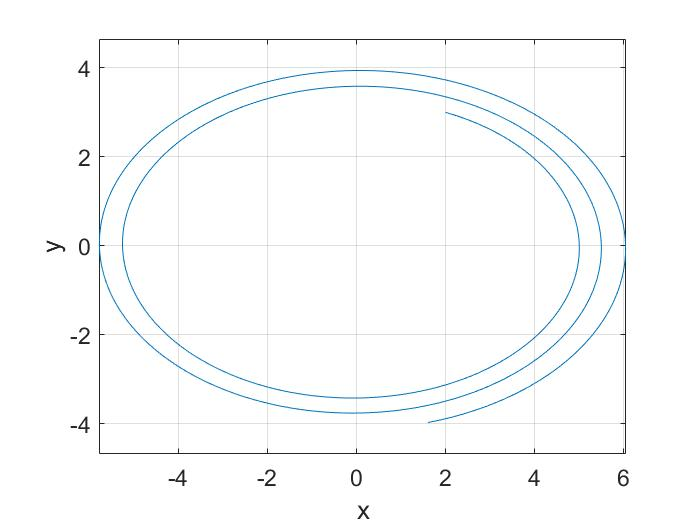
\includegraphics[width=8cm]{ExplEular_2.jpg}
\caption{显式Eular法求得的相平面中的轨迹}\label{2_2}
\end{figure}

用隐式Eular法求解其数值解,相平面中的轨迹如图\ref{2_3},发现相平面中轨迹偏离。
\begin{figure}[h]
\centering
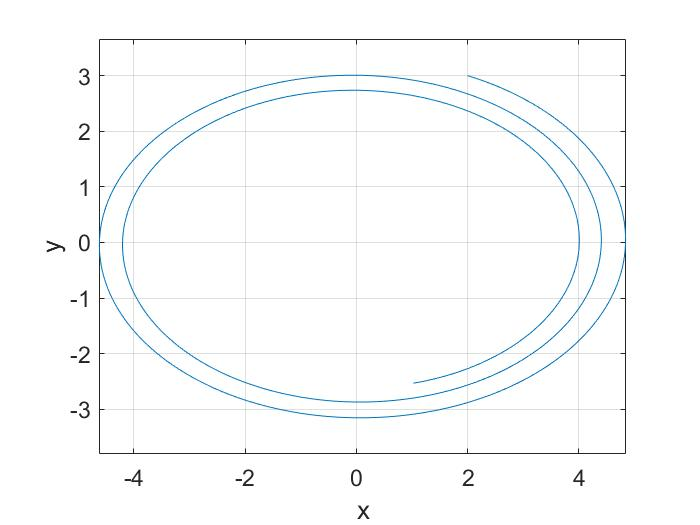
\includegraphics[width=8cm]{ImplEular_2.jpg}
\caption{隐式Eular法求得的相平面中的轨迹}\label{2_3}
\end{figure}

用四阶Runge--Kutta法求解其数值解,相平面中的轨迹如图\ref{2_4},发现相平面中轨迹轻微偏离(由于图片质量问题,图中显示不明显)。
\begin{figure}[h]
\centering
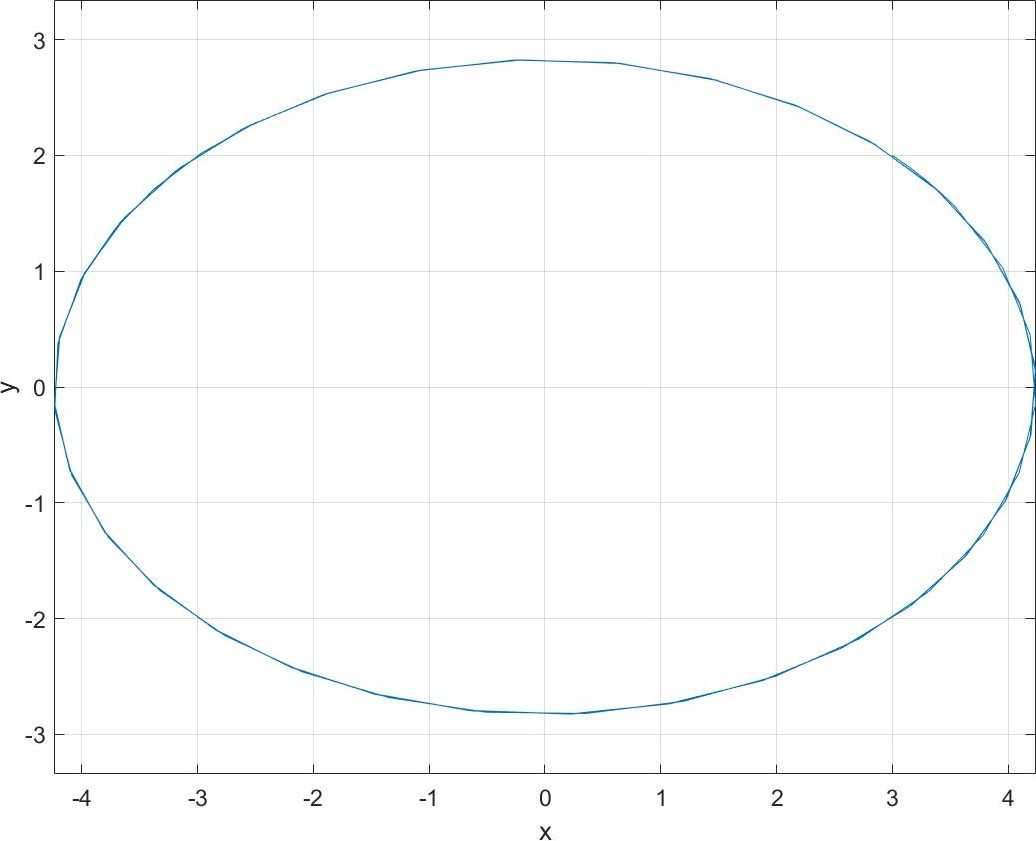
\includegraphics[width=12cm]{Runge_Kutta_2.jpg}
\caption{四阶Runge--Kutta法求得的相平面中的轨迹}\label{2_4}
\end{figure}

综上,只有梯形法求得的结果能保持相平面中的轨迹不变。

\section*{三、体会非线性方程的迭代求解}
用隐式欧拉公式和梯形公式求下单摆问题
\[
\left\{\begin{array}{ll}
\frac{d^2\theta(t)}{dt^2}+\sin\theta=0,&0<t\leq10\\
\theta(0)=\frac{\pi}{3}\\
\frac{d\theta}{dt}|_{t=0}=-\frac{1}{2}
\end{array}\right.
\]
取步长$h=0.02$. 取迭代误差$\varepsilon=10^{-6}$. 绘出近似解的图形.\\
解:将问题转化为一阶常微分方程组
\[
\left\{\begin{array}{ll}
y'(t)=z(t),&0<t\leq10\\
z'(t)=-\sin y(t),&0<t\leq10\\
y(0)=\frac{\pi}{3}\\
z(0)=-\frac{1}{2}
\end{array}\right.
\]
用隐式欧拉公式求解(Seidel型迭代格式),
\[
\left\{\begin{array}{l}
y_{n+1}^{(k+1)}=y_n+hz_{n+1}^{(k)}\\
z_{n+1}^{(k+1)}=z_n-h\sin y_{n+1}^{(k+1)}
\end{array}\right.
\]
结果如图\ref{3_1}。
\begin{figure}[h]
\centering
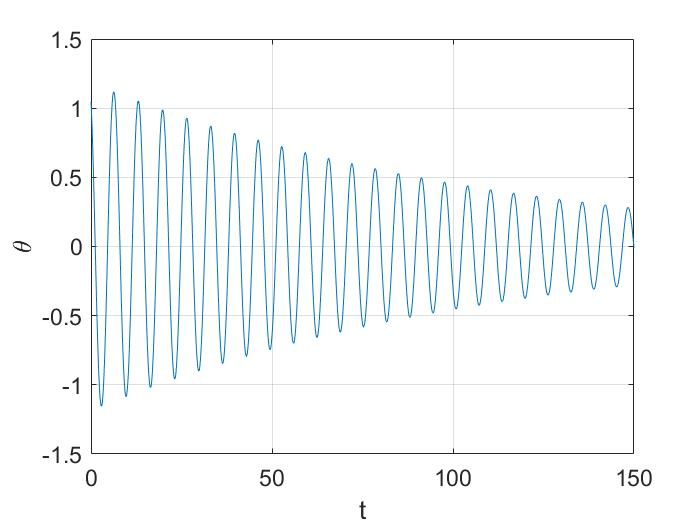
\includegraphics[width=8cm]{ImplEular_3.jpg}
\caption{隐式欧拉法求得的$\theta$--$t$曲线}\label{3_1}
\end{figure}

用梯形公式求解(Seidel型迭代格式),
\[
\left\{\begin{array}{l}
y_{n+1}^{(k+1)}=y_n+\frac{h}{2}(z_n+z_{n+1}^{(k)})\\
z_{n+1}^{(k+1)}=z_n+\frac{h}{2}(\sin y_n+\sin y_{n+1}^{(k+1)})
\end{array}\right.
\]
结果如图\ref{3_2}。
\begin{figure}[h]
\centering
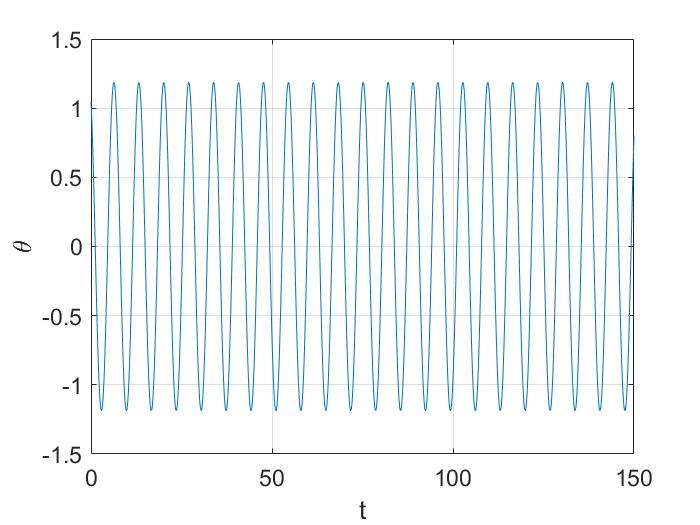
\includegraphics[width=8cm]{Trapezoid_3.jpg}
\caption{梯形法求得的$\theta$--$t$曲线}\label{3_2}
\end{figure}

\section*{MATLAB代码}
一、1.显式欧拉法
\begin{lstlisting}
close all;clear;clc;
h = 0.05;
x = 0:0.01:0.4;
y = 100;
analyticalsol = y * exp(-50 .* x);
figure(1);
plot(x,analyticalsol,'-','LineWidth',2);
hold on;
x = 0:h:0.4;
analyticalsol = y * exp(-50 .* x);
for i = x(1:end - 1)
    y(end + 1) = y(end) + h * (-50 * y(end));
end
plot(x,y,'.','MarkerSize',20);
grid on;
xlabel('x');
ylabel('y');
legend('Analytical Solution y=100e^{-50x}','Numerical Solution','Interpreter','tex');
figure(2);
plot(1:size(x,2) - 1,abs(y(2:end) - analyticalsol(2:end)),'-','LineWidth',2);
grid on;
xlabel('Iteration times n');
ylabel('The absolute of the error |\epsilon_n|','Interpreter','tex');
\end{lstlisting}
二、梯形法
\begin{lstlisting}
close all;clear;clc;
h = 0.01;
t = 0:h:5;
yx = [3;2]; 
for i = t
    yx(:,end + 1) = inv(eye(2) - h * [0 -2;9/2 0]) * (eye(2) + h * [0 -2;9/2 0]) * yx(:,end);
end
plot(yx(2,:),yx(1,:));
grid on;
axis equal;
xlabel('x');
ylabel('y');
\end{lstlisting}
显式Eular法
\begin{lstlisting}
close all;clear;clc;
h = 0.01;
t = 0:h:5;
yx = [3;2]; 
for i = t
    yx(:,end + 1) = yx(:,end) + h * [0 -2;9/2 0] * yx(:,end);
end
plot(yx(2,:),yx(1,:));
grid on;
axis equal;
xlabel('x');
ylabel('y');
\end{lstlisting}
隐式Eular法
\begin{lstlisting}
close all;clear;clc;
h = 0.01;
t = 0:h:5;
yx = [3;2]; 
for i = t
    yx(:,end + 1) = inv(eye(2) - h * [0 -2;9/2 0]) * yx(:,end);
end
plot(yx(2,:),yx(1,:));
grid on;
axis equal;
xlabel('x');
ylabel('y');
\end{lstlisting}
四阶Runge--Kutta法
\begin{lstlisting}
close all;clear;clc;
[T,YX] = ode45('f2',[0 10],[2;3]);
plot(YX(:,2),YX(:,1));
grid on;
axis equal;
xlabel('x');
ylabel('y');
function dyx = f2(t,yx)
dyx = [-2 * yx(2);9/2 * yx(1)];
end
\end{lstlisting}
三、隐式欧拉法
\begin{lstlisting}
close all;clear;clc;
h = 0.02;
epsilon = 10^(-6);
t = 0:h:20;
yz = [pi / 3;-1 / 2]; 
for i = t(1:end - 1)
    y0 = yz(1,end) + h * yz(2,end);
    z0 = yz(2,end) - h * sin(yz(1,end));
    y = yz(1,end) + h * z0;
    z = yz(2,end) - h * sin(y);
    while norm([y - y0;z - z0],inf) > epsilon
        y0 = y;
        z0 = z;
        y = yz(1,end) +  h * z0;
        z = yz(2,end) - h * sin(y);
    end
    yz(:,end + 1) = [y;z];
end
plot(t,yz(1,:));
grid on;
axis equal;
xlabel('t');
ylabel('\theta','Interpreter','tex');
\end{lstlisting}
梯形法
\begin{lstlisting}
close all;clear;clc;
h = 0.02;
epsilon = 10^(-6);
t = 0:h:20;
yz = [pi / 3;-1 / 2]; 
for i = t(1:end - 1)
    y0 = yz(1,end) + h * yz(2,end);
    z0 = yz(2,end) - h * sin(yz(1,end));
    y = yz(1,end) + h / 2 * (yz(2,end) + z0);
    z = yz(2,end) - h / 2 * (sin(yz(1,end)) + sin(y));
    while norm([y - y0;z - z0],inf) > epsilon
        y0 = y;
        z0 = z;
        y = yz(1,end) + h / 2 * (yz(2,end) + z0);
        z = yz(2,end) - h / 2 * (sin(yz(1,end)) + sin(y));
    end
    yz(:,end + 1) = [y;z];
end
plot(t,yz(1,:));
grid on;
axis equal;
xlabel('t');
ylabel('\theta','Interpreter','tex');
\end{lstlisting}
\end{document}